\documentclass[11pt,a4paper]{article}
\usepackage[T1]{fontenc}
\usepackage[utf8]{inputenc}
\usepackage{lmodern,microtype}
\usepackage{amsmath,amssymb,amsthm,mathtools,bm}
\usepackage{booktabs,array,tabularx,longtable}
\usepackage{graphicx,float,caption}
\usepackage{xcolor}
\usepackage[margin=20mm]{geometry}
\usepackage{enumitem,fancyhdr}
\usepackage[hidelinks,unicode=true]{hyperref}
\hypersetup{
 pdftitle={FIN ST118--ST129: Operational Equivalence, Certified Design, and Typed Tests},
 pdfauthor={Krzysztof Żuchowski},
 pdfsubject={Analytical and computational execution of FIN programs ST118--ST129},
 pdfkeywords={FIN, operational equivalence, observable algebra, lift polyhedron, Krawczyk replay, recoverable code, active pump, Chernoff design, correlated nuisance, thermal operations}
}
\setlength{\parindent}{0pt}
\setlength{\parskip}{0.48em}
\setlength{\emergencystretch}{2em}
\setlength{\headheight}{14pt}
\setlist[itemize]{leftmargin=1.55em,itemsep=0.14em,topsep=0.2em}
\setlist[enumerate]{leftmargin=1.75em,itemsep=0.14em,topsep=0.2em}
\pagestyle{fancy}\fancyhf{}
\lhead{FIN ST118--ST129}\rhead{Release 10.64}\cfoot{\thepage}
\newtheorem{theorem}{Theorem}[section]
\newtheorem{proposition}[theorem]{Proposition}
\newtheorem{corollary}[theorem]{Corollary}
\newcommand{\proven}{\textcolor{green!40!black}{\textbf{[PROVEN]}}}
\newcommand{\strong}{\textcolor{blue!70!black}{\textbf{[STRONG EVIDENCE]}}}
\newcommand{\conditional}{\textcolor{violet!65!black}{\textbf{[CONDITIONAL]}}}
\newcommand{\openstatus}{\textcolor{red!72!black}{\textbf{[OPEN]}}}
\newcommand{\statusboundary}{\textcolor{orange!80!black}{\textbf{[BOUNDARY]}}}
\newcommand{\resultbox}[1]{\begin{center}\fcolorbox{blue!60!black}{blue!4}{\parbox{0.92\textwidth}{#1}}\end{center}}

\begin{document}
\pagenumbering{gobble}
\begin{titlepage}
\centering
\vspace*{1.0cm}
{\LARGE\bfseries FIN ST118--ST129\par}
\vspace{0.32cm}
{\Large Operational Equivalence, Certified Design, and Typed Tests\par}
\vspace{0.42cm}
{\large A universal fine-blind quotient, exact circulant lift geometry, an independent transcendental-fold replay, complete maximal-code normal forms, invariant-state nonselection, a minimal pumped bifurcation, local interval certification of continuous design, mixed refinements, gauge-net locality, correlated-noise impossibility, a typed thermal subclass, and minimax fine observation\par}
\vspace{0.82cm}
{\Large Krzysztof \.{Z}uchowski\par}
\vspace{0.20cm}
{\large Independent Researcher --- Fractal Information Theory Project\par}
{\large ORCID: 0009-0002-0909-3613\par}
\vspace{0.62cm}
{\large FIN Release 10.64 --- Version 1.0.0\par}
{\large August 11, 2026\par}
\vfill
\begin{minipage}{0.91\textwidth}
\textbf{Question.} Can a precise operational equivalence select the fine-blind algebra; how much hidden-lift geometry, recoverability, active amplification, robust design, refinement, and thermodynamic separation follows once every additional premise is typed?\par
\textbf{Methods.} Fixed-point operator algebras, Haar twirling, exact diagonally-dominant polyhedra, independent interval Krawczyk replay, Knill--Laflamme theory, equivariant-state no-go arguments, scalar bifurcation theory, two-variable interval certification, refinement parity, information-theoretic counterexamples, and finite dilation witnesses.\par
\textbf{Epistemic rule.} Exact finite results, constructed conditional models, sampled evidence, and unresolved interval obligations are reported separately. No mathematical quotient is promoted to an observed universe.\par
\textbf{Repository snapshot.} Audited tracked base commit \texttt{8a4c9b0b29b4fed8f7dcdc86e79b98306818efea}; Release 10.64 artifacts are identified by a separate SHA-256 manifest.\par
\textbf{Repository.} \url{https://github.com/hyconiek/Fractal-Nadsoliton-Theory}\par
\textbf{License.} CC BY 4.0.
\end{minipage}
\end{titlepage}
\pagenumbering{arabic}

\begin{abstract}
ST118--ST129 continue the falsification-first analysis of the FIN projection architecture. ST118 supplies the mathematically smallest explicit equivalence relation that yields the fine-blind observable algebra. If arbitrary changes of basis in the twelve-dimensional fine sector are operational gauge, the fixed-point algebra is $M_{12}\oplus\mathbb C$ and Haar twirling gives its unique trace-preserving expectation. The result is exact but conditional: the fine gauge equivalence is the missing axiom, not a consequence of the strict operator. ST126 repackages it as a gauge-fixed local net and proves that locality still does no selecting work without the gauge premise.

ST119 exactly classifies the real symmetric circulant section of the complete 78-dimensional lift fiber. Positivity follows from diagonal dominance, and the section is
\[
[s,\infty)\times\prod_{d=1}^{6}[-w_d,w_d].
\]
It has $2^6=64$ vertices and one recession ray. This is a complete seven-parameter classification, not a classification of all noncirculant faces. ST120 independently reproduces the ST108 transcendental-kernel Krawczyk inclusion using only NumPy and mpmath, without SciPy or FIN research modules. It also corrects a precision description: the internal evaluation uses 70 decimal digits, but conversion to outward binary64 bounds produces kernel widths of approximately one binary64 ulp, $10^{-16}$--$10^{-18}$, not serialized widths of order $10^{-70}$.

ST121 proves a complete normal form for every maximal twelve-dimensional code recoverable after coarse/fine pinching. ST122 proves that all normalized positive strict functional-calculus states remain uniform under a covariant twelve-branch instrument and therefore cannot provide the missing selector. ST123 constructs the minimal scalar pumped pitchfork and writes its pump/dissipation/saturation balance explicitly; active information gain requires a supplied pump and clock.

ST124 obtains a strict two-variable Krawczyk certificate for the stationary Chernoff design near $\beta=2.1861899250$, $s=0.5398337033$. A radius-$10^{-6}$ box has inclusion margin $9.9983\times10^{-7}$. However, 274 boxes remain unresolved in the attempted global interval derivative cover. A 2,001-point audit finds one sign change, but global uniqueness is retained only as strong numerical evidence. ST125 proves the mixed-degree refinement parity theorem.

ST127 gives a sharp impossibility theorem: one-event marginals and detector-error bounds do not imply a positive finite-count error exponent under arbitrary temporal correlations. ST128 constructs a covariant Gibbs-preserving reset channel outside a precisely declared zero-Hamiltonian-bath thermal subclass; it does not separate CGP from standard thermal operations with energy-bearing baths. ST129 proves that the unique diagonal minimax detector against the normalized adversarial lift simplex is $P_f/12$, guaranteeing response $1/12$. The batch strengthens the conditional operational model while leaving the fine-gauge source, QW-2191, dimensions, and physical apparatus open.
\end{abstract}

\textbf{Status vocabulary.} \proven{} denotes an exact analytic, finite, or source-code interval theorem in its stated scope. \strong{} denotes stable numerical evidence. \conditional{} requires explicitly displayed resources. \openstatus{} marks an unclosed goal. \statusboundary{} records a non-implication.

\tableofcontents
\newpage

\section{Frozen core and research boundary}

The working strict operator remains
\begin{equation}
W_{xx}=0,\qquad W_{xy}=w_{d(x,y)}=\frac{\cos(0.18575d(x,y)+0.16250)}{1+d(x,y)^{9/5}}\quad(x\ne y),
\qquad A=sI-W,
\label{eq:strict}
\end{equation}
with $s=2\sum_{d=1}^{5}w_d+w_6$. The twelve declared weights are positive in the finite domain, so $A\succeq0$. The coarse/fine isometries are
\[
P=2^{-1/2}\binom I I,\qquad F=2^{-1/2}\binom I{-I},
\qquad P^*P=F^*F=I,\quad P^*F=0.
\]

The legacy ontological kernel remains an intermediate bridge kernel. No calculation below identifies it with~\eqref{eq:strict} or transfers its proposed physical roles. The nadsoliton is retained as the primordial informational object in solitonic state; no lower informational medium is inserted.

\resultbox{\textbf{Central conclusion.} The desired fine-blind algebra has a clean universal construction, but only after arbitrary fine-sector basis changes are declared operational gauge. The mathematics now identifies the missing axiom exactly; it still does not derive that axiom, a selector, or an apparatus from strict $A$.}

\section{Outcome matrix}
\small
\begin{longtable}{@{}p{0.065\textwidth}p{0.27\textwidth}p{0.27\textwidth}p{0.31\textwidth}@{}}
\toprule ID & Target & Result & Boundary\\\midrule\endfirsthead
\toprule ID & Target & Result & Boundary\\\midrule\endhead
ST118 & Operational equivalence & \proven{} universal fixed algebra & Fine gauge remains an axiom\\
ST119 & Circulant lift faces & \proven{} $64$ vertices plus one ray & Noncirculant faces unclassified\\
ST120 & Minimal ST108 replay & \proven{} independent two-dependency replay & Numerical center remains input\\
ST121 & Maximal codes & \proven{} complete graph-code normal form & $\alpha$ and unitaries unselected\\
ST122 & Strict-derived state selector & \proven{} invariant-state no-go & Noninvariant source remains absent\\
ST123 & Minimal active extension & \proven{} pumped scalar pitchfork & Pump, clock, units supplied\\
ST124 & Continuous design & \proven{} local stationary root; \strong{} global & 274 global cover boxes unresolved\\
ST125 & Mixed refinement & \proven{} parity theorem & Degrees and twists supplied\\
ST126 & Alternative locality & \proven{} conditional gauge net & Gauge, not locality, selects\\
ST127 & Correlated nuisance & \proven{} no count exponent in general & Mixing/independence needed\\
ST128 & CGP versus typed TO & \proven{} restricted separation & Standard TO separation open\\
ST129 & Minimax fine detector & \proven{} $P_f/12$, value $1/12$ & Cone and detector budget supplied\\
\bottomrule
\end{longtable}
\normalsize

\section{ST118 and ST126: the precise missing operational axiom}

Let the fine-sector gauge group be
\[
G_f=\{I_c\oplus U_f:U_f\in U(12)\}.
\]
It acts by conjugation on $M_{24}$.

\begin{theorem}[Fine-blind fixed algebra]
The fixed-point algebra of $G_f$ is
\[
M_{24}^{G_f}=P M_{12}P^*\oplus\mathbb CP_f.
\]
Its trace-preserving conditional expectation is
\[
E(X)=P_cXP_c+\frac{\operatorname{Tr}(P_fXP_f)}{12}P_f.
\]
\end{theorem}

\textit{Proof.} Every cross-sector block transforms under a nontrivial defining representation and must vanish. The coarse block is unaffected. A fine block commuting with every $U(12)$ is scalar by Schur's lemma. Haar averaging gives the displayed expectation. \hfill$\square$

This is a universal operational statement: if all gauge-invariant states and instruments agree on two observables, their images under $E$ agree; conversely the fixed algebra separates the equivalence classes. Two necessity tests are exact. Weakening $G_f$ to layer swap returns $M_{12}\oplus M_{12}$; deleting fine gauge and admitting vertex resolution generates $M_{24}$.

ST126 defines a coarse local net
\[
\mathcal A(O)=P M_O P^*\oplus\mathbb CP_f.
\]
It is isotone, and declared disjoint coarse regions commute when their coarse matrix algebras commute. Yet its global algebra is fine-blind only because $G_f$ was inserted. A causal or local vocabulary does not remove this source premise.

\begin{figure}[H]\centering
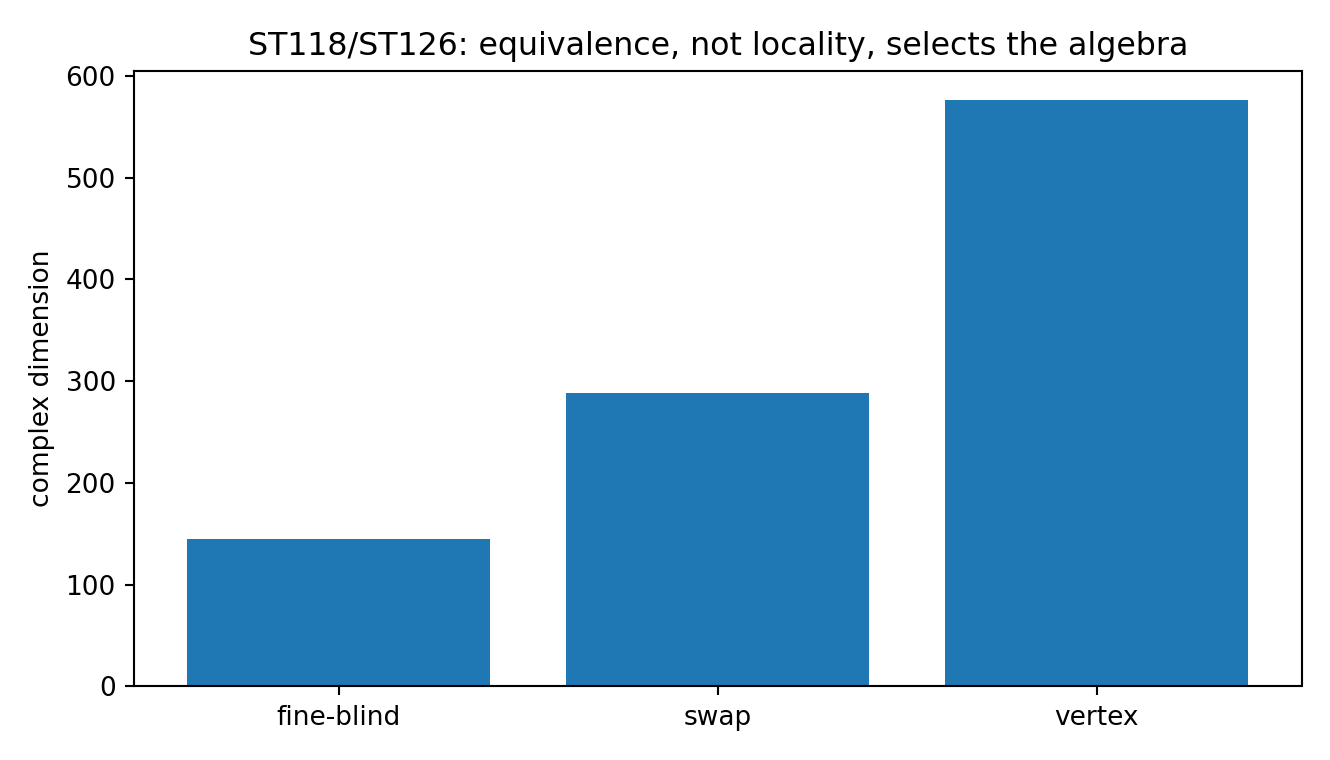
\includegraphics[width=.75\textwidth]{FIN_ST118_ST129_Figures/st118_equivalence_algebras.png}
\caption{ST118/ST126. Fine gauge equivalence selects dimension 145; swap symmetry and vertex locality select larger algebras.}
\end{figure}

\openstatus{} The next strict question is whether $G_f$ arises from an operational indistinguishability theorem independent of naming the fine sector. Current strict functional calculus does not provide it.

\section{ST119: complete circulant geometry of the hidden lift fiber}

Every real symmetric circulant fine block is determined by
\[
B=\operatorname{circ}(b_0,b_1,b_2,b_3,b_4,b_5,b_6,b_5,b_4,b_3,b_2,b_1).
\]
The complete graph bounds inherited from ST95 become
\[
b_0\ge s,\qquad -w_d\le b_d\le w_d\quad(d=1,\ldots,6).
\]

\begin{theorem}[Exact circulant lift polyhedron]
Every point satisfying these coordinate inequalities is positive semidefinite. Hence the complete circulant section is
\[
\mathcal F_{\rm circ}=[s,\infty)\times\prod_{d=1}^{6}[-w_d,w_d].
\]
It has exactly $64$ vertices, $b_0=s$ and $b_d=\pm w_d$, and one recession extreme ray in the positive $b_0$ direction.
\end{theorem}

\textit{Proof.} The absolute off-diagonal row sum is at most $2\sum_{d=1}^{5}w_d+w_6=s\le b_0$. Thus $B$ is symmetric diagonally dominant with nonnegative diagonal and is positive semidefinite. The remaining polyhedral statement is the vertex/ray structure of one half-line times a six-cube. \hfill$\square$

\begin{figure}[H]\centering
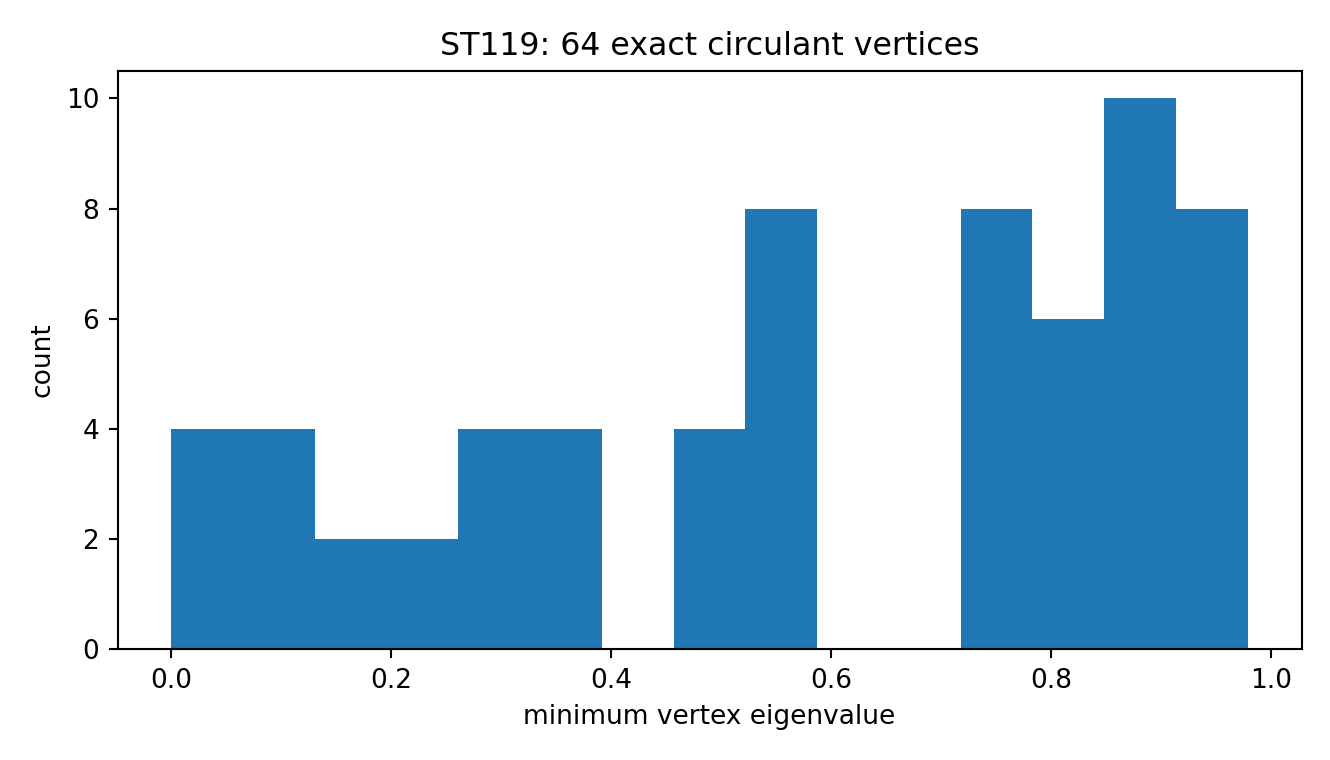
\includegraphics[width=.73\textwidth]{FIN_ST118_ST129_Figures/st119_vertices.png}
\caption{ST119. Binary64 spectral checks of the 64 analytically classified vertices; tiny negative minima are roundoff around zero.}
\end{figure}

The result completely solves the seven-parameter cyclic section but not the entire 78-dimensional noncirculant spectrahedron.

\section{ST120: independent replay and precision correction}

The standalone replay \texttt{fin\_st120\_minimal\_replay.py} imports only NumPy and mpmath beyond the Python standard library. It imports neither SciPy nor any FIN research module. Starting from the published 15-variable numerical center, it independently reconstructs:
\begin{enumerate}
\item the outward transcendental kernel intervals;
\item the fold equations and all 225 interval Jacobian entries;
\item the midpoint inverse and interval matrix products;
\item four Krawczyk boxes.
\end{enumerate}

\begin{theorem}[Independent replay]
The radius-$10^{-8}$ box is strictly included with margin
\[
9.999987060638205\times10^{-9}.
\]
All four tested radii pass, reproducing ST108 without its project import chain or SciPy solver.
\end{theorem}

\begin{figure}[H]\centering
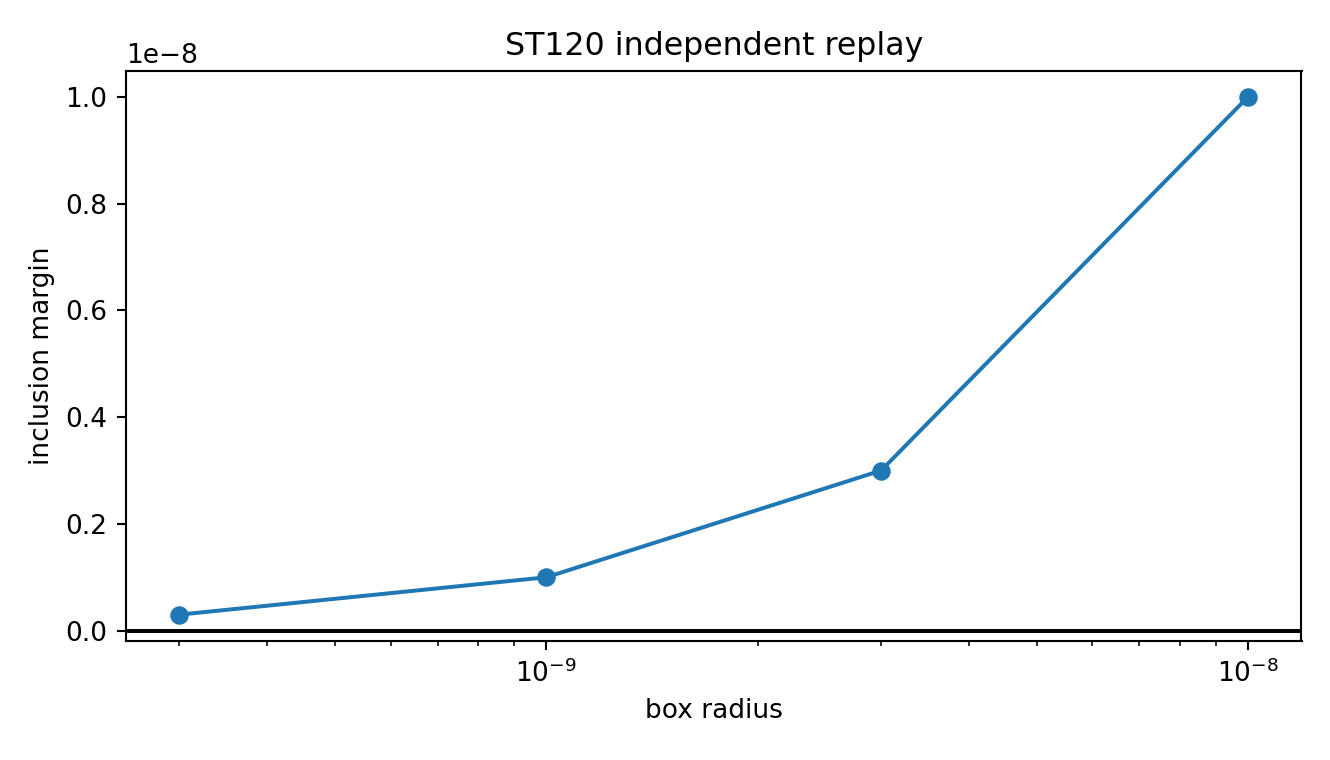
\includegraphics[width=.72\textwidth]{FIN_ST118_ST129_Figures/st120_replay.png}
\caption{ST120. Independently recomputed strict inclusion margins.}
\end{figure}

\textbf{Precision correction.} The transcendental evaluation is performed at 70 decimal digits. When its endpoints are deliberately converted to outward binary64 bounds for the matrix proof, the stored widths become approximately one ulp: $1.11\times10^{-16}$ for $w_1$, down to $3.47\times10^{-18}$ for $w_6$. Release 10.63's statement that retained widths were of order $10^{-70}$ was imprecise; it described the internal decimal evaluation rather than the actual exported float enclosure. The inclusion theorem is unaffected because the wider binary64 enclosure is the one used in the Krawczyk calculation.

\statusboundary{} The numerical center remains a supplied input. ST132 is intended to replace it with an independent interval-Newton center-isolation stage.

\section{ST121: all maximal recoverable codes}

For pinching errors $P_c,P_f$, a code projector $Q$ is correctable iff
\[
QP_cQ=\alpha Q,\qquad QP_fQ=(1-\alpha)Q.
\]

\begin{theorem}[Maximal-code normal form]
Every correctable code of maximal dimension twelve has one of the following forms:
\begin{align*}
\alpha=1 &: \quad \operatorname{Ran}Q=\operatorname{Ran}P,\\
\alpha=0 &: \quad \operatorname{Ran}Q=\operatorname{Ran}F,\\
0<\alpha<1 &: \quad V\psi=\sqrt\alpha\,PU_c\psi+\sqrt{1-\alpha}\,FU_f\psi,
\end{align*}
where $U_c,U_f\in U(12)$. Conversely every displayed code is exactly recoverable.
\end{theorem}

\textit{Proof.} For $0<\alpha<1$, the normalized restrictions $\alpha^{-1/2}P_c|_Q$ and $(1-\alpha)^{-1/2}P_f|_Q$ are isometries between equal twelve-dimensional spaces and hence unitaries. The endpoint cases occupy a full sector. Direct substitution proves the converse. \hfill$\square$

Up to independent sector unitaries the continuous invariant is $\alpha$. Neither $\alpha$ nor the two unitaries is selected by strict $A$.

\section{ST122: strict invariant states cannot break the branch symmetry}

Let $\rho=f(A)/\operatorname{Tr}f(A)$ with $f(A)\succeq0$. Since $A$ commutes with the cyclic and reflection representations, so does $\rho$.

\begin{theorem}[Functional-calculus nonselection]
For every covariant twelve-outcome vertex instrument, every strict functional-calculus state has the uniform outcome law $p_x=1/12$. Therefore no state in this class supplies a nonuniform branch measure, orientation, or selector.
\end{theorem}

The proof is transitivity: invariance gives $p_x=p_{g x}$ for every $g\in C_{12}$; normalization gives $1/12$. Numerical Gibbs checks for $\beta=0,0.2,0.8,2,8$ have maximum deviations below $1.6\times10^{-16}$.

\statusboundary{} A noninvariant initial state, boundary state, instrument, or environment evades the theorem by supplying the missing symmetry-breaking object. QW-2191 remains open.

\section{ST123: the smallest honest active extension contains a pump}

Consider
\begin{equation}
\dot x=(g-\gamma)x-\kappa x^3+u,\qquad y=x,
\label{eq:pump}
\end{equation}
with $\gamma,\kappa>0$. For $V=x^2/2$,
\[
\dot V=gx^2-\gamma x^2-\kappa x^4+uy.
\]

\begin{theorem}[Pumped pitchfork and cost balance]
For $g\le\gamma$, $x=0$ is stable and there is no nonzero self-amplified equilibrium. At $g=\gamma$ a pitchfork occurs. For $g>\gamma$, the stable equilibria are
\[
x_\pm=\pm\sqrt{\frac{g-\gamma}{\kappa}}.
\]
At either equilibrium the pump injection equals dissipation plus saturation.
\end{theorem}

\begin{figure}[H]\centering
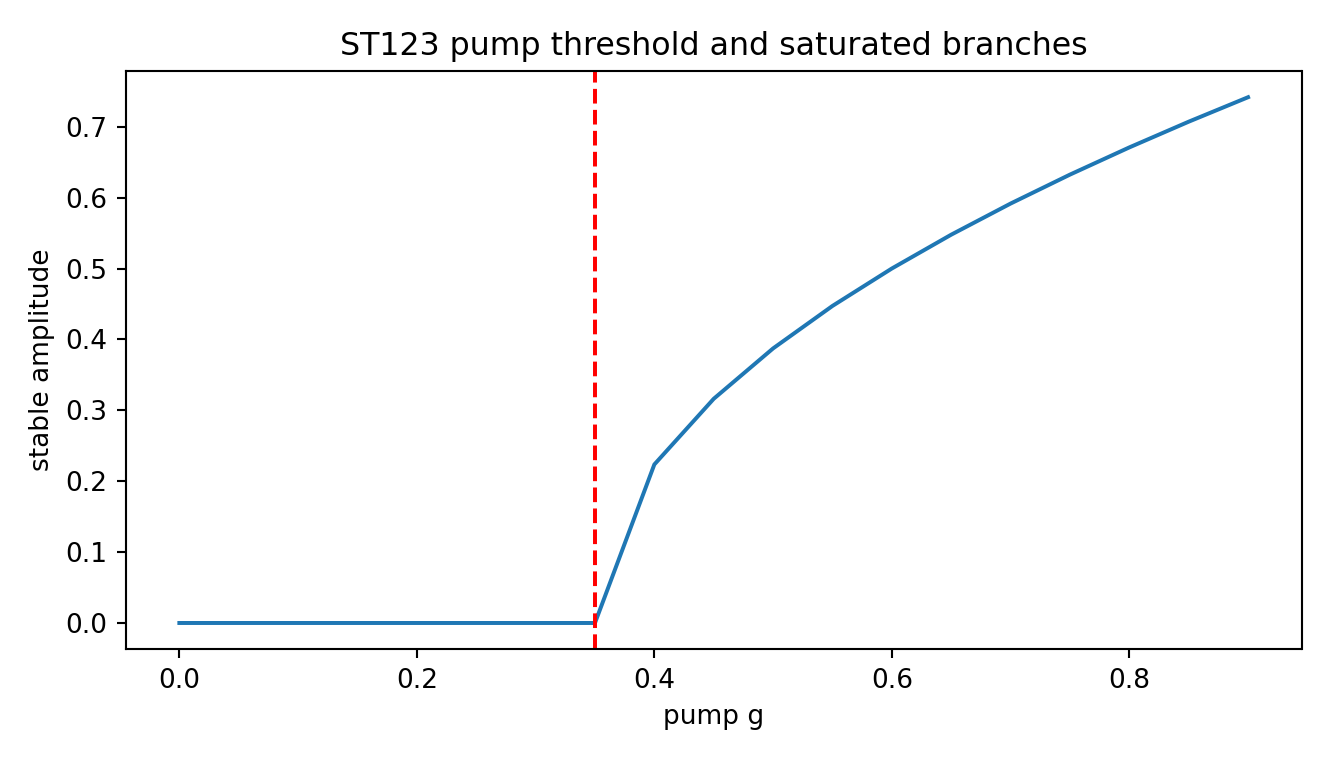
\includegraphics[width=.73\textwidth]{FIN_ST118_ST129_Figures/st123_active_threshold.png}
\caption{ST123. A self-amplified branch appears only after the explicit pump crosses the loss threshold.}
\end{figure}

This separates symmetry from positive feedback. Symmetry supplies the pair $x_\pm$; the pump creates the instability and the cubic term saturates it. The model is constructed. Its clock, $g$, $\gamma$, $\kappa$, and energetic units are not generated by FIN.

\section{ST124: local interval theorem, global claim withheld}

For hypotheses $q_0=0.2$, $q_1=0.7$ and symmetric detector flip $\delta=0.05$, let $B_s(\beta)$ be the Bernoulli Chernoff coefficient. An interior optimum obeys
\[
\partial_s B_s=0,\qquad \partial_\beta B_s=0.
\]
The code evaluates partition functions and their first two derivatives from the outward-enclosed binary64 spectra. A two-variable Krawczyk operator then encloses the stationary system.

\begin{theorem}[Local stationary design]
There is exactly one solution inside the radius-$10^{-6}$ box centered at
\[
(\beta_*,s_*)=(2.186189925005268,\ 0.539833703306343).
\]
The strict inclusion margin is $9.9983368\times10^{-7}$ and
\[
C(\beta_*)\in[0.04073095991295749,\ 0.04073095991295826].
\]
\end{theorem}

\begin{figure}[H]\centering
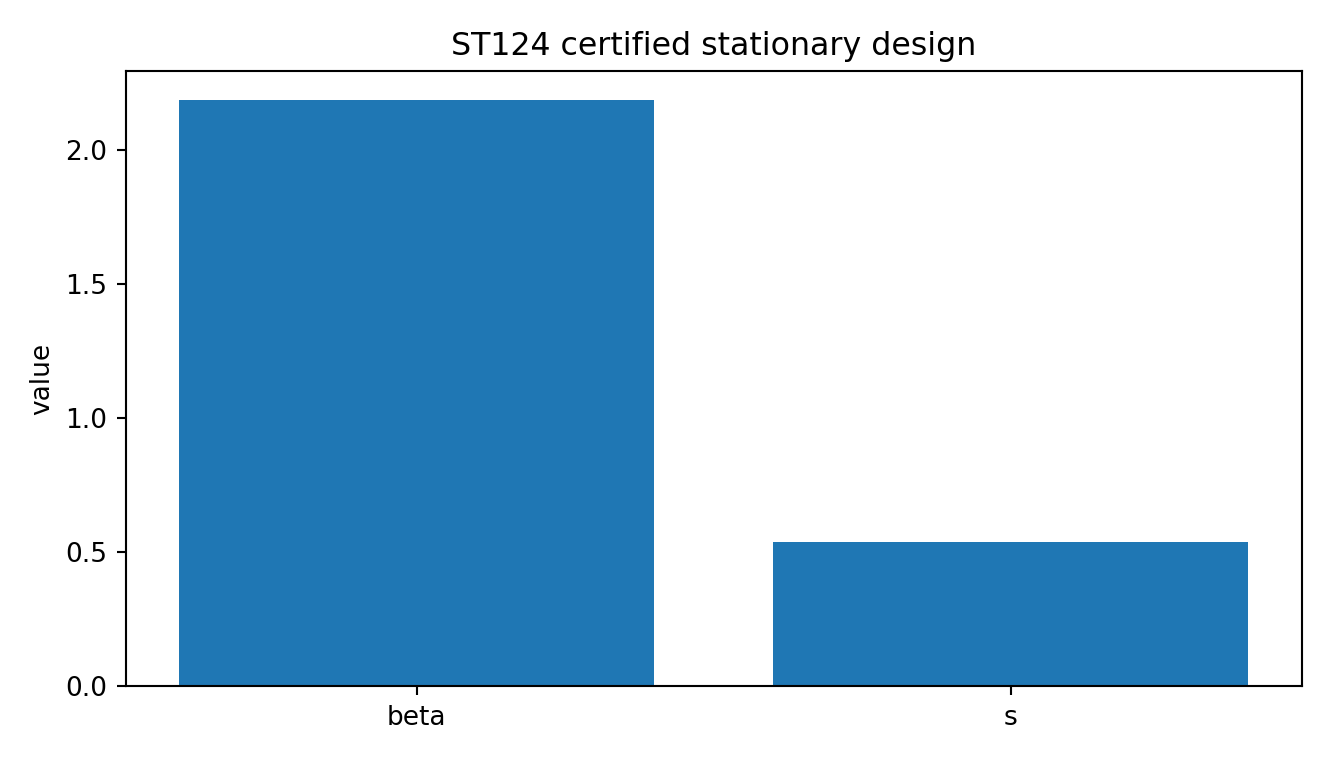
\includegraphics[width=.68\textwidth]{FIN_ST118_ST129_Figures/st124_beta_certificate.png}
\caption{ST124. Center of the certified two-variable stationary box.}
\end{figure}

The attempted global proof subdivided $\beta\in[0.05,5]$ and tested the sign of the envelope derivative outside the root box. It certified 99 boxes but left 274 unresolved because interval dependency made the closed-form Chernoff exponent ill-conditioned, especially near nearly equal distributions. A separate 2,001-point floating audit found exactly one sign change.

\strong{} The point is the apparent unique global maximum on the declared domain. \openstatus{} Global interval uniqueness is not proved. The report deliberately does not convert the dense audit into a theorem.

\section{ST125: parity controls mixed-degree holonomy}

For a degree-$m$ cover, $\mathbb Z_2$ holonomy pulls back as
\[
h\longmapsto h^m.
\]

\begin{theorem}[Mixed-refinement parity]
Odd degrees preserve $h$. Every even degree maps both signs to $+1$. In an untwisted mixed tower, an initial antiperiodic class survives exactly until the first even degree and can never reappear afterward. With twists,
\[
h_{n+1}=t_nh_n^{m_n},
\]
so recovery after an even step is newly supplied data.
\end{theorem}

\begin{figure}[H]\centering
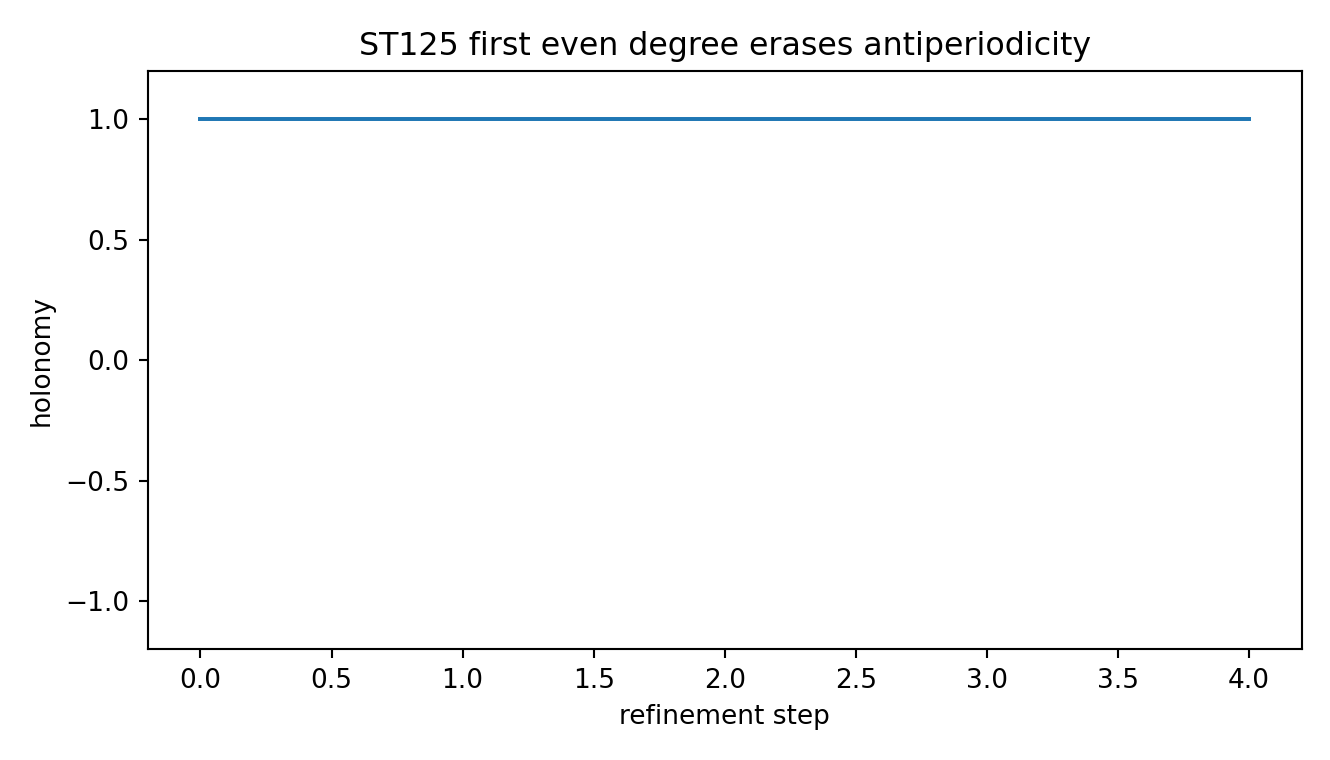
\includegraphics[width=.72\textwidth]{FIN_ST118_ST129_Figures/st125_mixed_refinement.png}
\caption{ST125. The first even refinement erases untwisted antiperiodicity in the example tower.}
\end{figure}

No physical spin or fermion source follows from this combinatorial classification.

\section{ST127: arbitrary temporal correlation destroys event-count scaling}

Suppose the one-event distributions under two hypotheses are Bernoulli$(p_0)$ and Bernoulli$(p_1)$. Draw one latent variable $Y$ under the relevant hypothesis and report
\[
X_1=X_2=\cdots=X_n=Y.
\]
Each event has the declared marginal for every $n$, but the complete record contains one independent bit.

\begin{theorem}[No positive exponent from marginals alone]
One-event marginals and detector-error bounds do not imply a positive asymptotic discrimination exponent under arbitrary temporal correlation. In the construction above, the equal-prior Bayes error is
\[
P_e^{(n)}=\frac12(1-|p_1-p_0|)
\]
for every $n$.
\end{theorem}

\begin{figure}[H]\centering
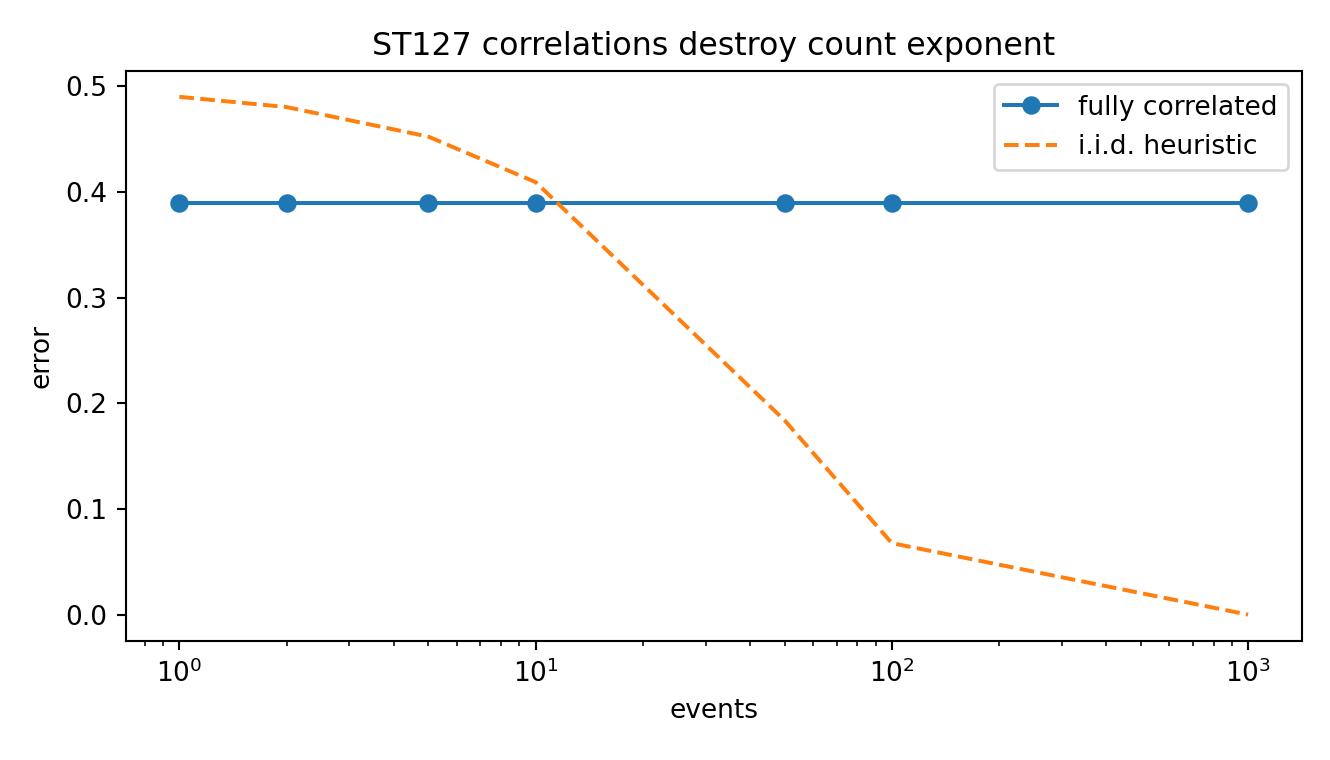
\includegraphics[width=.72\textwidth]{FIN_ST118_ST129_Figures/st127_correlated_nuisance.png}
\caption{ST127. Fully correlated events retain the one-event error while an i.i.d. heuristic decreases exponentially.}
\end{figure}

This does not invalidate ST115's single-joint-event Chernoff theorem. It invalidates automatic multiplication of that information by an event count unless independence, Markov mixing, or another dependence bound is separately certified.

\section{ST128: an exact but deliberately restricted thermal separation}

Declare the bath class to consist of arbitrary finite-dimensional baths with
\[
H_B=0,\qquad[U,H_S\otimes I_B]=0.
\]
Let $\gamma_\beta=e^{-\beta H_S}/Z$ and define the reset channel
\[
\Phi_\gamma(\rho)=\gamma_\beta\operatorname{Tr}\rho.
\]

\begin{theorem}[Typed restricted separation]
$\Phi_\gamma$ is CPTP, Gibbs preserving, and time-translation covariant. It cannot be implemented by any dilation in the declared $H_B=0$ class.
\end{theorem}

\textit{Proof.} A permitted unitary commutes with every system spectral projector and therefore preserves every system energy-block population for every input. The reset channel changes those populations unless they are already Gibbs. \hfill$\square$

\statusboundary{} This proves CGP is larger than one explicitly declared zero-energy-bath subclass. It does not prove $\mathrm{CGP}\setminus\mathrm{TO}\ne\varnothing$ for the standard class with energy-bearing baths, catalysts, approximate implementations, or unbounded ancillas.

\section{ST129: exact minimax fine observation}

Normalize the adversarial recession directions to
\[
\Delta L(t)=F\operatorname{diag}(t)F^*,\qquad t_i\ge0,\quad\sum_i t_i=1.
\]
Under the detector budget
\[
H(h)=F\operatorname{diag}(h)F^*,\qquad h_i\ge0,\quad\sum_i h_i=1,
\]
the response is $\operatorname{Tr}[H(h)\Delta L(t)]=h\cdot t$.

\begin{theorem}[Unique diagonal minimax detector]
\[
\max_{h\in\Delta_{11}}\min_{t\in\Delta_{11}}h\cdot t=\frac1{12}.
\]
The unique maximizer is $h_i=1/12$, hence $H=P_f/12$.
\end{theorem}

\textit{Proof.} The inner minimum is $\min_i h_i$. Since $\sum_i h_i=1$, this is at most $1/12$, with equality only for the uniform vector. \hfill$\square$

\begin{figure}[H]\centering
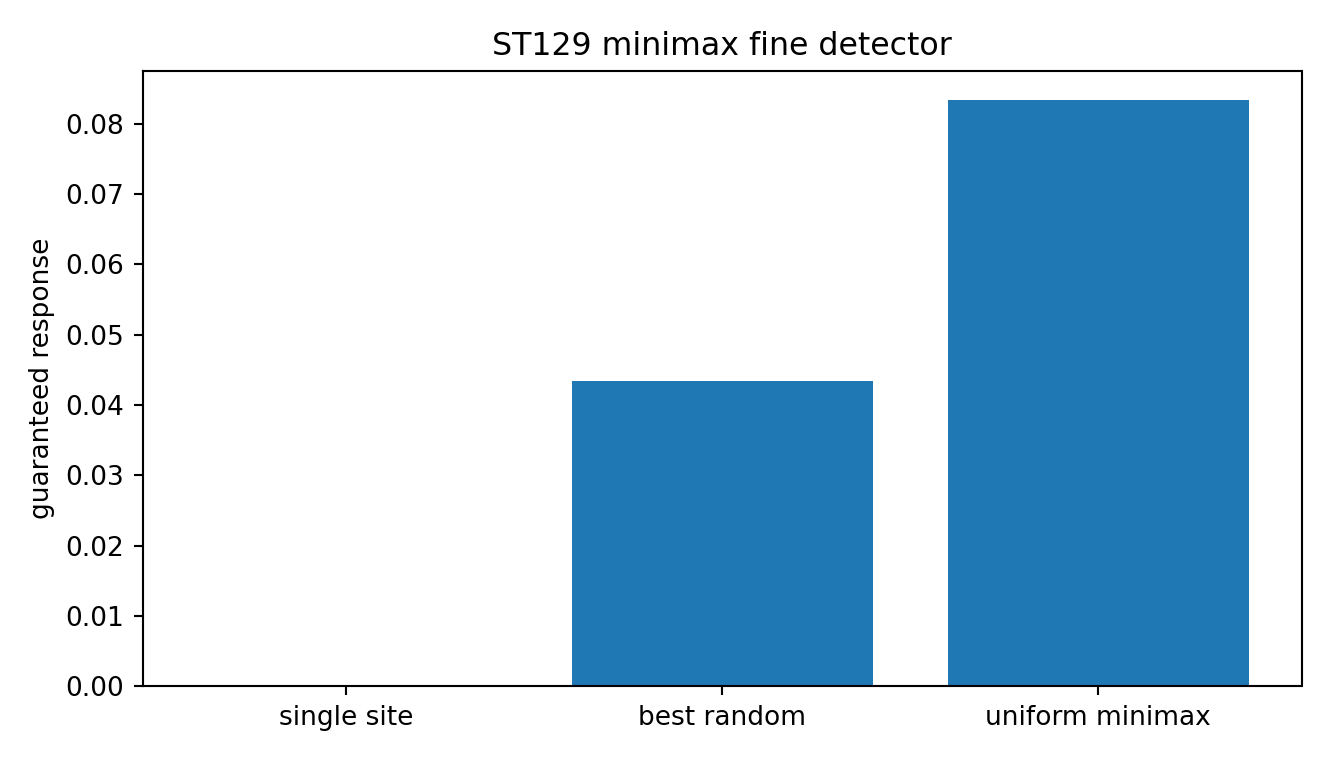
\includegraphics[width=.70\textwidth]{FIN_ST118_ST129_Figures/st129_minimax_detector.png}
\caption{ST129. Uniform fine observation dominates single-site and random budget allocations in worst-case response.}
\end{figure}

Every coarse observable has zero response. A single-site fine detector also has worst-case response zero because the adversary can choose another site. The result is conditional on the normalized cone and detector budget; it is not a laboratory POVM design.

\section{Failed approaches and corrected claims}

\begin{enumerate}
\item \textbf{Locality still did not derive fine blindness.} The gauge-net construction works because a fine gauge was declared.
\item \textbf{Strict invariant states did not produce spontaneous branch weights.} Every covariant record stayed uniform.
\item \textbf{Active gain did not emerge from antisymmetry.} The smallest successful construction required an explicit pump and saturation.
\item \textbf{The continuous design was not globally interval-certified.} A strict local root exists, but interval dependency left 274 boxes unresolved.
\item \textbf{One-event nuisance robustness did not imply finite-count robustness.} Arbitrary temporal correlation eliminated the exponent.
\item \textbf{Thermal strictness depended on the declared bath.} A restricted separation was proved; the standard-class question remains open.
\item \textbf{A precision sentence from Release 10.63 was corrected.} The proof used outward binary64 ulps, not stored $10^{-70}$-wide float intervals.
\end{enumerate}

\section{Recommended programs ST130--ST141}

\small
\begin{longtable}{@{}p{0.07\textwidth}p{0.57\textwidth}p{0.26\textwidth}@{}}
\toprule Priority & Program & Success criterion\\\midrule\endfirsthead
\toprule Priority & Program & Success criterion\\\midrule\endhead
1 & \textbf{ST130}: strict source or no-go for fine $U(12)$ gauge equivalence & Source theorem independent of naming fine sector\\
2 & \textbf{ST131}: noncirculant low-rank faces of the full lift fiber & Certified new face family beyond the six-cube\\
3 & \textbf{ST132}: remove imported ST108 center & Independent interval-Newton center isolation\\
4 & \textbf{ST133}: recovery under noisy pinching & Optimal fidelity/code theorem\\
5 & \textbf{ST134}: minimal-rank symmetry-breaking states & Typed source cost or no-go\\
6 & \textbf{ST135}: couple the pump to strict modes & Existence/stability without physical promotion\\
7 & \textbf{ST136}: interval detector and $q$ uncertainty & Uniform local/global design certificate\\
8 & \textbf{ST137}: arbitrary refinement diagrams & Path-independent twist/cocycle classification\\
9 & \textbf{ST138}: causal conditional independence & Algebra selection without pre-naming fine sector\\
10 & \textbf{ST139}: certified dependent-count bounds & Markov or $\alpha$-mixing error exponent\\
11 & \textbf{ST140}: one matched-gap bath qubit & Exact dilation feasibility beyond $H_B=0$\\
12 & \textbf{ST141}: noisy non-diagonal minimax design & Optimal observable on a bounded full-face class\\
\bottomrule
\end{longtable}
\normalsize

\section{Reproducibility}

The executable package contains:
\begin{itemize}
\item \texttt{fin\_st118\_st129\_research.py} and 28-test validation suite;
\item dependency-minimal \texttt{fin\_st120\_minimal\_replay.py};
\item full results and summary ledgers;
\item ST119, ST120, ST124, and ST129 certificate/packet JSON files;
\item eight generated figures and a SHA-256 manifest.
\end{itemize}

The main script uses Python 3.12, NumPy, SciPy, mpmath interval arithmetic, and Matplotlib. The standalone ST120 replay uses only NumPy and mpmath as third-party dependencies. The command
\[
\texttt{python3 -m unittest -v test\_fin\_st118\_st129.py}
\]
passes all 28 tests. Live tests reconstruct lift vertices, Knill--Laflamme identities, pump balance, interval inclusion, refinement parity, constant correlated error, and the minimax detector.

\section{Final verdict}

\resultbox{\textbf{Verdict surviving ST118--ST129.} FIN now has a precise conditional answer to ``what is the projection?'': it is the fixed algebra of an explicit fine-sector gauge equivalence. The answer is mathematically minimal and operationally coherent, but the equivalence itself remains the missing principle. Hidden lift freedom is exactly large even in the cyclic section; strict invariant states cannot select a branch; active gain requires a pump; finite-count claims require dependence control; and thermal separation is bath-class dependent. The theory has become more sharply falsifiable without becoming experimentally established physics.}

The most important next question is ST130: can the fine gauge equivalence be obtained without naming it in advance, from a strict operational indistinguishability or redundancy theorem? A negative theorem would be scientifically valuable: it would prove that the projection layer is irreducibly additional rather than merely undiscovered.

\begin{thebibliography}{9}
\bibitem{Krawczyk} R. Krawczyk, ``Newton-Algorithmen zur Bestimmung von Nullstellen mit Fehlerschranken,'' \emph{Computing} 4 (1969), 187--201.
\bibitem{KnillLaflamme} E. Knill and R. Laflamme, ``Theory of quantum error-correcting codes,'' \emph{Physical Review A} 55 (1997), 900--911.
\bibitem{Chernoff} H. Chernoff, ``A measure of asymptotic efficiency for tests of a hypothesis based on the sum of observations,'' \emph{Annals of Mathematical Statistics} 23 (1952), 493--507.
\bibitem{BratteliRobinson} O. Bratteli and D. W. Robinson, \emph{Operator Algebras and Quantum Statistical Mechanics I}, Springer, second edition, 1987.
\end{thebibliography}

\end{document}
